
\section{Experimental Evaluation}
\label{sec:experiments}

We evaluate polynomial hashing constructions over the finite field $\mathbb{F}_{2^{64}}$
in two distinct settings:
\begin{enumerate}
    \item \textbf{$k$-wise independent hashing} (Section~\ref{sec:experiments:kwise}):
          The polynomial coefficients are random \emph{keys}, and we hash a single data point $x$.
          Applications include hash tables, load balancing, and randomized algorithms
          requiring bounded independence.
    \item \textbf{Universal hashing} (Section~\ref{sec:experiments:universal}):
          The polynomial evaluation point(s) are random \emph{keys}, and we hash a
          variable-length \emph{message}.
          Applications include message authentication codes (MACs), checksums,
          and data structure fingerprinting.
\end{enumerate}
The key distinction is key size: $k$-wise hashing uses $O(k)$ keys to hash one value,
while universal hashing uses $O(1)$ keys to hash messages of any length.

\subsection{Experimental Setup}

We benchmark on two platforms:
\begin{itemize}
    \item \textbf{ARM}: Apple M1 Pro (ARM64) running macOS, using ARM NEON intrinsics
          for carryless multiplication via the \texttt{PMULL} instruction.
    \item \textbf{x86}: AMD EPYC 9R14 (x86-64) running Linux, using Intel intrinsics
          for carryless multiplication via the \texttt{PCLMULQDQ} instruction.
\end{itemize}
Both instructions compute the product of two 64-bit polynomials over $\mathbb{F}_2$
using dedicated hardware support.

We compare the following evaluation methods, all operating over $\mathbb{F}_{2^{64}}$:
\begin{itemize}
    \item \textbf{Horner}: Standard Horner's rule with carryless multiplication
          and full polynomial reduction after each step.
          For a monic degree-$n$ polynomial (with $n$ coefficient keys), this requires $n-1$ multiplications
          executed sequentially.
    \item \textbf{Lemire}: Horner's rule using Lemire's fast modular reduction~\cite{lemire2019fast},
          which replaces one of the three \texttt{PMULL} operations in the Barrett reduction
          with a 256-byte table lookup.
    \item \textbf{Estrin}: Estrin's parallel evaluation scheme~\cite{estrin1960organization},
          which groups coefficients into pairs and evaluates them in parallel.
          This exposes instruction-level parallelism but requires computing powers
          $x^2, x^4, \ldots$, increasing the total multiplication count.
    \item \textbf{Rabin--Winograd}: The recursive divide-and-conquer method of
          Rabin and Winograd~\cite{rabin1972number}, which splits a polynomial
          into two halves and evaluates them with shared intermediate values.
          This achieves $\lceil n/2 \rceil + O(\log n)$ multiplications.
    \item \textbf{This Paper}: Our optimized polynomial chains,
          using the minimum number of multiplications for each degree
          as described in this paper.
\end{itemize}

Each algorithm was benchmarked by hashing $10^6$ random 64-bit integers,
repeated 100 times. We report mean$\pm$standard deviation; figures show $\pm 1$ standard deviation error bars.
With 100 repetitions, the $95\%$ confidence interval for the mean is approximately $\pm 0.2\cdot\text{std}$.
We measure evaluation time only; key setup and preprocessing (when applicable) are excluded.

\paragraph{Platform scope.}
We report results for both ARM (Apple M1 Pro) and x86 (AMD EPYC 9R14).
The qualitative trade-offs (depth vs.\ total multiplications, and the cost of modular reduction)
are consistent across platforms, though quantitative speedups vary with microarchitecture.

\paragraph{Reproducibility.}
The ARM benchmarks are in \texttt{tools/bench/\allowbreak carryless\_arm.cpp}, compiled with
\texttt{Apple clang 17.0.0} using \texttt{-O3 -std=c++17 -march=armv8-a+crypto}.
The x86 benchmarks are in \texttt{tools/bench/\allowbreak carryless.cpp}, compiled with
\texttt{GCC 11.5.0} using \texttt{-O3 -std=c++17 -mpclmul -march=native}.
We use the same input sequence across methods and include a warmup phase before timing.

\paragraph{Implementation Details.}
Our ARM implementation uses several key optimizations:
(1) Keys are stored as scalar 64-bit integers rather than 128-bit SIMD vectors,
    allowing XOR operations to use the faster scalar ALU;
(2) Modular reduction uses three \texttt{PMULL} operations rather than table lookup,
    which we found to be faster on Apple Silicon;
(3) Independent multiplication chains are interleaved to exploit instruction-level parallelism.

\subsection{\texorpdfstring{$k$}{k}-wise Independent Hashing}
\label{sec:experiments:kwise}

We evaluate the monic degree-$k$ polynomial family $h(x) = x^k + a_{k-1}x^{k-1} + \cdots + a_1 x + a_0$ over $\mathbb{F}_{2^{64}}$.
Here the $k$ coefficients $(a_0, \ldots, a_{k-1})$ are the random key, and we hash a single data point $x$.

\begin{figure}[!htbp]
    \centering
    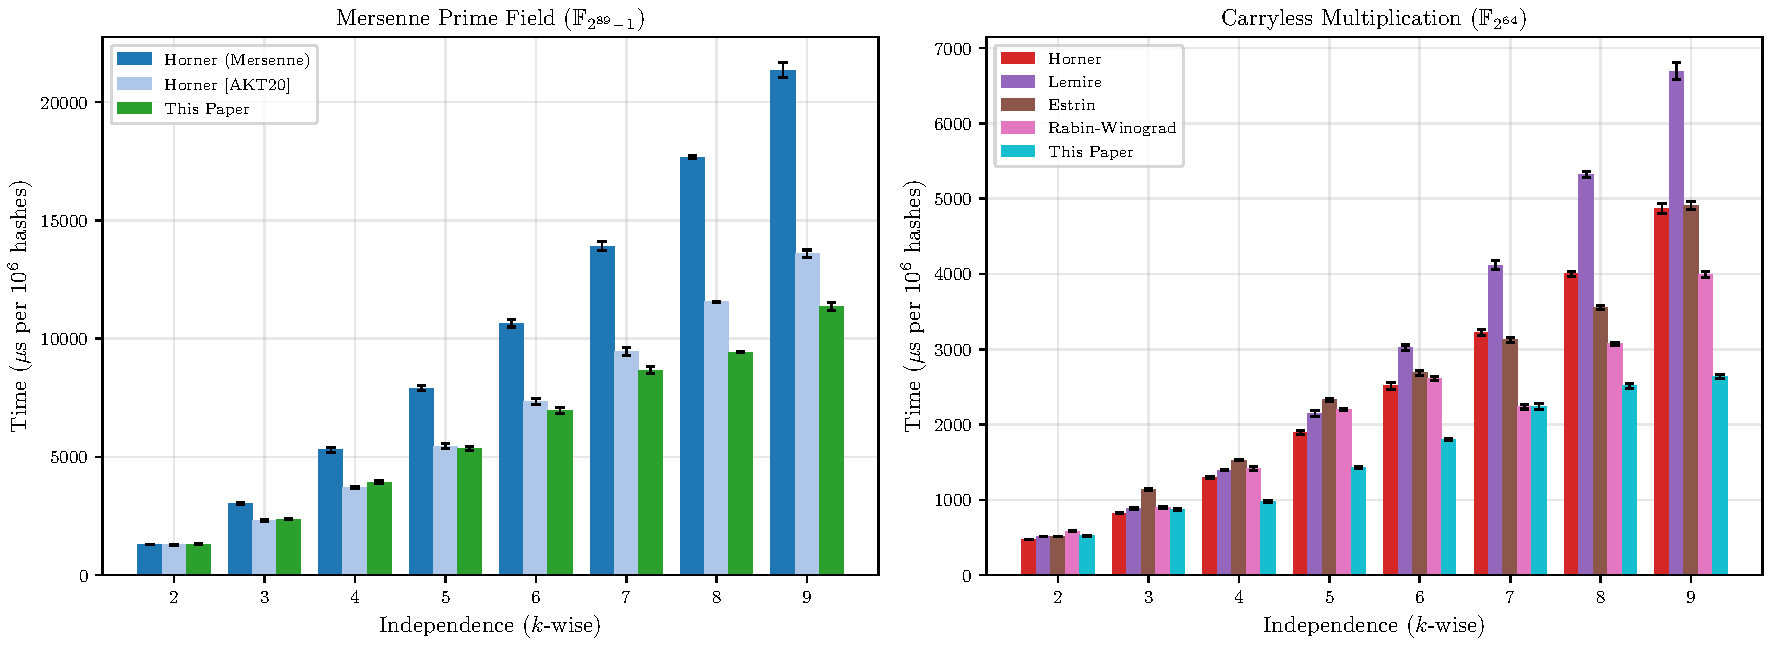
\includegraphics[width=\columnwidth]{figures/bench_all.pdf}
    \caption{Comparison across finite fields: Mersenne prime (left) vs.\
             carryless $\mathbb{F}_{2^{64}}$ (right).
             Carryless multiplication is $3$--$5\times$ faster due to
             hardware support via \texttt{PMULL}/\texttt{PCLMULQDQ}.}
    \label{fig:bench_all}
\end{figure}

Table~\ref{tab:kwise_both} shows the carryless hashing results on both platforms.
Our polynomial chains are the fastest method for most values of $k$, except at $k=7$ where Rabin--Winograd performs best.

\begin{table}[!htbp]
\centering
\caption{$k$-wise carryless hashing (\textmu s per $10^6$ hashes).
         Best method in bold for each platform.}
\label{tab:kwise_both}
\begin{tabular}{c|rrrrr|rrrrr}
    & \multicolumn{5}{c|}{ARM (Apple M1 Pro)} & \multicolumn{5}{c}{x86 (AMD EPYC 9R14)} \\
    $k$ & Horner & Lemire & Estrin & R--W & Ours & Horner & Lemire & Estrin & R--W & Ours \\
    \hline
    3 & 852 & 1144 & 1330 & 1537 & \textbf{914} & 3277 & \textbf{2198} & 3278 & 2281 & 2285 \\
    5 & 1931 & 2911 & 3075 & 3125 & \textbf{1521} & 6558 & 5653 & 6558 & 6140 & \textbf{4214} \\
    7 & 3354 & 5558 & 4002 & \textbf{2346} & 2346 & 10501 & 10005 & 8745 & \textbf{6236} & 6074 \\
    9 & 5188 & 9082 & 5856 & 4716 & \textbf{2833} & 14754 & 14489 & 12546 & 10300 & \textbf{7303} \\
\end{tabular}
\end{table}
For $k = 9$, our method achieves a speedup of $1.83\times$ over Horner on ARM and $2.02\times$ on x86.
For smaller $k$, we use Motzkin's method for $k=4$ (2 multiplications) and direct evaluation for $k=3$ (1 multiplication).
The speedup increases with $k$ because our polynomial chains save more multiplications
at higher degrees: for monic degree $n$, Horner uses $n-1$ multiplications while our
chains use only $\lfloor n/2\rfloor+1$ multiplications (by \cref{thm:main}).

\paragraph{Discussion.}
The Rabin--Winograd method performs best at $k = 7$ where its recursive structure
aligns well with the degree, achieving performance competitive with Estrin.
For other values of $k$, Rabin--Winograd is slower than our method but remains competitive
with standard approaches.
Estrin's scheme provides modest speedup at higher degrees due to its parallelism,
but the additional multiplications limit its effectiveness.
Lemire's reduction is slower than Horner because, on Apple Silicon,
the \texttt{PMULL} instruction is faster than table lookup operations.

Our method achieves the best performance by combining two key insights:
(1) minimizing the number of multiplications through carefully constructed polynomial chains,
and (2) optimizing the implementation to avoid unnecessary data movement between
scalar and vector registers.

On x86 (AMD EPYC 9R14), similar trends hold: our method achieves $2.02\times$ speedup
over Horner at $k=9$ (vs.\ $1.81\times$ on ARM).
Rabin--Winograd is competitive at $k=7$ on both platforms.
Notably, Lemire's table-lookup reduction is faster than Horner on x86,
unlike ARM where \texttt{PMULL} outperforms memory access.

\paragraph{Scope of application benchmarks.}
The remaining experiments measure end-to-end kernels where hashing is only one component.
These are representative workloads rather than an exhaustive study of all data structure designs and microarchitectures.

\subsection{Application-Level Throughput: Sketch Updates}
\label{sec:experiments:sketch}

To check that these savings translate beyond microbenchmarks, we also measure a simple
CountSketch-style update kernel: for each key, compute a hash value, use it to choose a bucket
and a sign bit, and update an array of counters.
This mixes hashing with memory traffic, so speedups are expected to be smaller than in the raw
hash-evaluation benchmark.

With table size $2^{16}$ and $2^{20}$ updates, we measure:
\begin{center}
\begin{tabular}{l|rrr|rrr}
& \multicolumn{3}{c|}{ARM} & \multicolumn{3}{c}{x86} \\
Method & Horner & R--W & Ours & Horner & R--W & Ours \\
\hline
ns/update & 5.49 & 4.96 & \textbf{4.33} & 38.3 & 24.9 & \textbf{23.7}
\end{tabular}
\end{center}
On ARM, our method achieves $1.27\times$ speedup over Horner.
On x86, the speedup is $1.62\times$, reflecting the larger benefit from reducing multiplications.
The benchmark is implemented in \texttt{tools/bench/\allowbreak app\_countsketch\_arm.cpp} (ARM) and
\texttt{tools/bench/\allowbreak app\_countsketch\_x86.cpp} (x86).

\subsection{Application-Level Throughput: Hash Tables}
\label{sec:experiments:hashtable}

Finally, we benchmark a simple linear-probing hash table, measuring both insertion throughput
(table construction) and lookup throughput at load factor $70\%$.
This stresses both hashing and memory probing; as expected, improvements are smaller than the
microbenchmarks, but still measurable.

With table size $2^{20}$, we obtain:
\begin{center}
\begin{tabular}{l|rrr|rrr}
& \multicolumn{3}{c|}{ARM} & \multicolumn{3}{c}{x86} \\
Method & Horner & R--W & Ours & Horner & R--W & Ours \\
\hline
ns/insert & 32.5 & 28.5 & \textbf{28.5} & 37.4 & 29.9 & \textbf{24.5} \\
ns/query  & 42.7 & 41.9 & \textbf{38.6} & 46.3 & 35.4 & \textbf{31.4}
\end{tabular}
\end{center}
On ARM, our method achieves $1.14\times$ speedup for inserts and $1.11\times$ for lookups.
On x86, speedups are larger: $1.53\times$ for inserts and $1.47\times$ for lookups.
The benchmark is implemented in \texttt{tools/bench/\allowbreak app\_linearprobe\_arm.cpp} (ARM) and
\texttt{tools/bench/\allowbreak app\_linearprobe\_x86.cpp} (x86).

\subsection{Application-Level Throughput: Membership Filters}
\label{sec:experiments:filter}

We also implement a simple XOR-filter-style approximate membership structure, which builds a
small fingerprint array using a peeling algorithm and answers queries with three table reads and
two XORs.
We measure both build throughput (ns/key) and query throughput (ns/query) at load $75\%$ and table
size $2^{20}$:
\begin{center}
\begin{tabular}{l|rrr|rrr}
& \multicolumn{3}{c|}{ARM} & \multicolumn{3}{c}{x86} \\
Method & Horner & R--W & Ours & Horner & R--W & Ours \\
\hline
ns/key (build) & 96.1 & \textbf{82.4} & 92.0 & 142.0 & 110.3 & \textbf{97.1} \\
ns/query       & 5.56 & 5.53 & \textbf{5.04} & 19.6 & 15.6 & \textbf{11.1}
\end{tabular}
\end{center}
On ARM, our method improves query throughput by $1.10\times$ over Horner, while R--W is faster at build time.
On x86, our method is fastest for both: $1.46\times$ speedup for build and $1.76\times$ for queries.
The benchmark is implemented in \texttt{tools/bench/\allowbreak app\_xorfilter\_arm.cpp} (ARM) and
\texttt{tools/bench/\allowbreak app\_xorfilter\_x86.cpp} (x86).

\subsection{Cryptographic Workloads: Secret Sharing and Polynomial PRFs}
\label{sec:experiments:crypto}

We also benchmark the same ``evaluate one random polynomial at many points'' inner loop that
appears in threshold secret sharing~\cite{shamir1979share} and related primitives.
To model prime-field arithmetic (where a multiplication is ``full width'' regardless of whether
the input happens to be a small integer), we use the Mersenne prime field
$\F_p$ with $p = 2^{89}-1$ and implement multiplication using 128-bit integer arithmetic and
Mersenne reduction.

We compare Horner evaluation against our ``x2s'' chains (degrees $13,15,17,19,21$ from our search)
in two regimes:
(1) ``Share generation'': evaluation points $x_i = i$ (but treated as elements of $\F_p$, so each
multiply is a full field multiplication), and
(2) ``Polynomial PRF'': evaluation points $x_i \sim \F_p$ uniformly at random.
Both correspond to real cryptographic use cases; the second is also a proxy for polynomial-based
PRFs / universal hashing keyed by the (preprocessed) coefficients.

On an Apple M1 Pro, we observe consistent $2.0\times$--$2.5\times$ speedups over full-field Horner
evaluation for degrees $13$--$21$ in both regimes; see the benchmark implementation in
\texttt{tools/bench/shamir\_sharegen\_mersenne.cpp}.
Including the cost of writing shares to memory gives essentially the same speedups; see
\texttt{tools/bench/shamir\_sharegen\_mersenne\_store.cpp}.

\begin{center}
\begin{tabular}{c|ccccc}
Degree $n$ & 13 & 15 & 17 & 19 & 21 \\
\hline
ARM: Sharegen ($x_i=i$) & 2.02$\times$ & 2.37$\times$ & 2.47$\times$ & 2.49$\times$ & 2.44$\times$ \\
ARM: PRF ($x_i \sim \F_p$) & 2.01$\times$ & 2.34$\times$ & 2.48$\times$ & 2.48$\times$ & 2.48$\times$ \\
\hline
x86: Sharegen ($x_i=i$) & 1.66$\times$ & 4.50$\times$ & 4.57$\times$ & 4.63$\times$ & 4.60$\times$ \\
x86: PRF ($x_i \sim \F_p$) & 1.66$\times$ & 4.50$\times$ & 4.57$\times$ & 4.63$\times$ & 4.60$\times$
\end{tabular}
\end{center}
On x86, the speedups for degrees $15$--$21$ reach $4.5\times$--$4.6\times$, significantly
exceeding the ARM results.

\paragraph{Goldilocks prime field.}
Prime fields of 64-bit size are widely used in proof systems; a common choice is the
``Goldilocks'' prime $p = 2^{64}-2^{32}+1$.
We repeat the same benchmark in $\F_p$ and observe similar improvements:
\begin{center}
\begin{tabular}{c|ccccc}
Degree $n$ & 13 & 15 & 17 & 19 & 21 \\
\hline
ARM: Sharegen ($x_i=i$) & 1.98$\times$ & 2.23$\times$ & 2.39$\times$ & 2.33$\times$ & 2.32$\times$ \\
ARM: PRF ($x_i \sim \F_p$) & 1.96$\times$ & 2.29$\times$ & 2.35$\times$ & 2.34$\times$ & 2.34$\times$ \\
\hline
x86: Sharegen ($x_i=i$) & 1.27$\times$ & 1.38$\times$ & 1.42$\times$ & 1.43$\times$ & 1.37$\times$ \\
x86: PRF ($x_i \sim \F_p$) & 1.27$\times$ & 1.38$\times$ & 1.42$\times$ & 1.43$\times$ & 1.37$\times$
\end{tabular}
\end{center}
The benchmark is implemented in \texttt{tools/bench/\allowbreak app\_goldilocks\_stark\_eval.cpp}.
On ARM, including memory stores gives $2.19\times$--$2.36\times$ speedup;
on x86, the range is $1.31\times$--$1.90\times$.
The smaller x86 gains reflect that Goldilocks multiplication (64-bit) is relatively cheaper,
reducing the benefit of fewer multiplications.
\par\noindent\texttt{tools/bench/\allowbreak app\_goldilocks\_sharegen\_store.cpp} contains the benchmark.

\subsection{Comparison with Tabulation Hashing}

Tabulation hashing~\cite{patracscu2012power} achieves 3-wise independence using
table lookups, providing excellent performance for applications that only require
low independence.
On ARM, simple tabulation (8 tables of 256 entries) achieves
1660$\pm$12\,\textmu s per $10^6$ hashes; on x86, it achieves 6952$\pm$5\,\textmu s.

Notably, our 3-wise independent hash function runs in 914$\pm$4\,\textmu s on ARM---nearly $2\times$ faster than
tabulation with the same independence guarantee.
On x86, our method (2285\,\textmu s) is $3\times$ faster than tabulation.
Our 4-wise hash (using Motzkin's method) is still faster than 3-wise tabulation on both platforms.

\begin{center}
\begin{tabular}{l|rr|rr}
    & \multicolumn{2}{c|}{ARM} & \multicolumn{2}{c}{x86} \\
    Method & Time (\textmu s) & Indep. & Time (\textmu s) & Indep. \\
    \hline
    MurmurHash3 & 593$\pm$8 & none & 1042$\pm$2 & none \\
    xxHash64 & 1174$\pm$5 & none & 1862$\pm$4 & none \\
    Tabulation & 1660$\pm$12 & 3-wise & 6952$\pm$5 & 3-wise \\
    This Paper ($k=3$) & 914$\pm$4 & 3-wise & 2285$\pm$3 & 3-wise \\
    This Paper ($k=4$) & 1036$\pm$13 & 4-wise & 3930$\pm$4 & 4-wise \\
    This Paper ($k=5$) & 1521$\pm$8 & 5-wise & 4214$\pm$3 & 5-wise \\
    This Paper ($k=7$) & 2346$\pm$9 & 7-wise & 6074$\pm$4 & 7-wise \\
\end{tabular}
\end{center}

\subsection{Comparison Across Finite Fields}

We also benchmark polynomial evaluation over the Mersenne prime field
$\mathbb{F}_{2^{89}-1}$, which uses 89-bit integers and standard multiplication
with modular reduction (Figure~\ref{fig:bench_all}).
For the Mersenne baseline, we use the optimized Horner implementation
from Ahle et al.~\cite{ahle2020power}, which employs fast branch-free
modular reduction and delays the final reduction to the end of the computation.
The carryless multiplication methods over $\mathbb{F}_{2^{64}}$ are consistently
$3$--$5\times$ faster than their Mersenne counterparts.
This speedup comes from hardware support for carryless multiplication (via \texttt{PMULL} on Apple M1 Pro),
which computes a 64-bit carryless product directly,
whereas Mersenne arithmetic requires multiple standard multiplications
and careful handling of the 89-bit modulus.

For $k=9$, our method over $\mathbb{F}_{2^{64}}$ (2833\,\textmu s mean) is
$4.2\times$ faster than the best Mersenne method in our benchmark (11864\,\textmu s mean).

\subsection{Injective Polynomial Hashing}
\label{sec:experiments:injective}

We briefly summarize the injective polynomial construction from Section~\ref{sec:injective}
before the comprehensive comparison in Section~\ref{sec:experiments:universal}.
The recurrence
\[
    P_0 = x, \quad P_i = a_i + (b_i + y)(P_{i-1} + x^2)
\]
uses only two random keys $(x, y)$ to hash $2N$ message values $(a_1, b_1, \ldots, a_N, b_N)$
with $N$ multiplications---half the $2N-1$ required by Horner.

\begin{table}[!htbp]
\centering
\caption{Injective vs.\ Horner: $N$ multiplications vs.\ $2N-1$.
         Times in \textmu s per $10^6$ hashes (mean$\pm$std).}
\label{tab:injective}
\begin{tabular}{c|rrr|rrr}
    & \multicolumn{3}{c|}{ARM (Apple M1 Pro)} & \multicolumn{3}{c}{x86 (AMD EPYC 9R14)} \\
    $2N$ & Horner & Injective & Speedup & Horner & Injective & Speedup \\
    \hline
    8  & 5560$\pm$20 & 3960$\pm$30 & $1.40\times$ & 16115$\pm$6 & 13672$\pm$6 & $1.18\times$ \\
    16 & 21030$\pm$160 & 9950$\pm$50 & $2.11\times$ & 48811$\pm$41 & 30413$\pm$9 & $1.61\times$ \\
    32 & 73720$\pm$240 & 40430$\pm$70 & $1.82\times$ & 134847$\pm$15 & 66778$\pm$27 & $2.02\times$ \\
    64 & 226910$\pm$940 & 114960$\pm$350 & $1.97\times$ & 310923$\pm$85 & 165921$\pm$27 & $1.87\times$ \\
\end{tabular}
\end{table}

The speedup approaches $2\times$ as expected from the multiplication count.
On x86, the gains are similar, ranging from $1.18\times$ at $2N=8$ to $2.02\times$ at $2N=32$.
For parallel variants and comparison with other methods (CLNH, BRW, etc.),
see Section~\ref{sec:experiments:universal}.

\subsection{Universal Hashing}
\label{sec:experiments:universal}

Universal hashing uses $O(1)$ random keys to hash variable-length messages.
Unlike $k$-wise hashing where polynomial coefficients are keys,
here the evaluation point(s) are keys and message values form the polynomial.
We compare several constructions, each offering different trade-offs between
key size, multiplication count, and parallelism.

\subsubsection{Horner-based Methods}

The simplest universal hash evaluates the polynomial
$h(x) = m_0 x^{n-1} + m_1 x^{n-2} + \cdots + m_{n-1}$
where $x$ is the random key and $(m_0, \ldots, m_{n-1})$ is the message.

\paragraph{Horner (Sequential).}
Horner's rule computes $h_0 = m_0$, $h_i = h_{i-1} \cdot x + m_i$ for $i = 1, \ldots, n-1$.
This requires $n-1$ multiplications with a \emph{critical path} of $n-1$ dependent operations.
On CPUs where multiplication has multi-cycle latency, this sequential
dependency chain leaves execution units idle.

\paragraph{Horner-Unrolled.}
We process four message values per iteration using Estrin-style grouping:
\[
h \cdot x^4 + (m_i \cdot x + m_{i+1}) \cdot x^2 + (m_{i+2} \cdot x + m_{i+3}).
\]
The terms $(m_i \cdot x + m_{i+1})$ and $(m_{i+2} \cdot x + m_{i+3})$ can be computed
in parallel, exposing instruction-level parallelism (ILP) within each 4-element group.
This reduces effective critical path by $\approx 4\times$ with minimal overhead.

\paragraph{Horner-Parallel.}
Horner's recurrence $h_i = h_{i-1} \cdot x + m_i$ is a linear map with transfer function
$(c, d) = (x, m_i)$, meaning $h \mapsto h \cdot c + d$.
Writing $T_{c,d}(h)\coloneqq h\cdot c + d$, composition is
\[
   T_{c_2,d_2}\!\circ T_{c_1,d_1} = T_{c_1c_2,\; d_1c_2 + d_2}.
\]
Since $c = x$ for all steps, we precompute powers $x, x^2, x^4, \ldots$ and combine
message values in a binary tree with $O(\log n)$ depth.
This requires $O(n)$ total multiplications but only $O(\log n)$ on the critical path.

\subsubsection{Injective Polynomial (This Paper)}

Our injective construction from Section~\ref{sec:injective} uses the recurrence:
\[
P_0 = x, \quad P_i = a_i + (b_i + y)(P_{i-1} + x^2).
\]
The message $(a_1, b_1, \ldots, a_N, b_N)$ has $2N$ values, and the keys are $(x, y)$---just
two field elements regardless of message length.
Each step requires one multiplication (computing $(b_i + y)(P_{i-1} + x^2)$),
so $N$ multiplications hash $2N$ values.
This is nearly $2\times$ fewer than Horner's $2N-1$ multiplications.

\paragraph{Injective-Parallel.}
The recurrence $P_i = a_i + c_i(P_{i-1} + x^2)$ where $c_i = b_i + y$ has transfer functions
$(c_i, d_i)$ with $d_i = a_i + c_i \cdot x^2$.
Unlike Horner, the coefficients $c_i$ vary, so we cannot simply precompute powers.
Instead, we compute all $(c_i, d_i)$ pairs in parallel (Phase~1: $N$ multiplications),
then perform parallel prefix reduction (Phase~2: $2N$ multiplications in $O(\log N)$ depth).
Total work is $3N$ multiplications, but critical path is only $O(\log N)$.

\subsubsection{CLNH (Multilinear Hashing)}

Carry-less NH (CLNH)~\cite{lemire2015clhash} is a multilinear hash:
\[
h = \bigoplus_{i=0}^{N-1} (k_{2i} \oplus m_{2i})(k_{2i+1} \oplus m_{2i+1})
\]
where $(k_0, \ldots, k_{2N-1})$ are random keys and $(m_0, \ldots, m_{2N-1})$ is the message.
All $N$ multiplications are \emph{completely independent}, giving $O(1)$ critical path depth.
This makes CLNH extremely fast on CPUs with multiple execution units.

\paragraph{Trade-off.}
CLNH requires $O(N)$ keys to hash an $N$-word message, compared to $O(1)$ for polynomial methods.
This is acceptable when key material can be generated once and reused (e.g., for a fixed
maximum message length), but problematic for variable-length or streaming applications.
We include CLNH as a performance baseline representing the ``best possible'' when key size
is unconstrained.

\subsubsection{BRW (Bernstein-Rabin-Winograd)}

The BRW construction~\cite{rabin1972number} uses divide-and-conquer to build a polynomial
with optimal $O(\log N)$ depth.
For a message $(m_1, \ldots, m_n)$, the BRW polynomial is defined recursively:
\begin{align}
\text{BRW}(m_1) &= m_1 \\
\text{BRW}(m_1, m_2) &= m_1 \cdot x + m_2 \\
\text{BRW}(m_1, m_2, m_3) &= (x + m_1)(x^2 + m_2) + m_3 \\
\text{BRW}(m_1, \ldots, m_{2^k-1}) &= \text{BRW}(\text{left}) \cdot (x^{2^{k-1}} + m_{2^{k-1}}) + \text{BRW}(\text{right})
\end{align}
This achieves $\approx n/2$ multiplications with $O(\log n)$ depth, which is asymptotically optimal up to lower-order terms~\cite{rabin1972number}.

\paragraph{Practical Limitation.}
Despite theoretical optimality, BRW performs poorly in practice.
The recursive structure with irregular base cases prevents effective compiler optimization.
Function call overhead and unpredictable branching inhibit instruction scheduling,
resulting in slower execution than simpler iterative methods.

\subsubsection{c-Decimated BRW}

To improve BRW's practical performance, $c$-decimated BRW splits the message into
$c$ interleaved streams, applies BRW to each stream, and combines results:
\[
h = \text{BRW}(m_0, m_c, m_{2c}, \ldots) + x^d \cdot \text{BRW}(m_1, m_{c+1}, \ldots) + \cdots
\]
where $d$ is chosen to avoid coefficient collisions.
The $c$ independent BRW evaluations can execute in parallel, improving ILP.
We benchmark $c = 2$ and $c = 4$.

\paragraph{Result.}
Even with decimation, BRW variants remain slower than Horner-Unrolled and Injective-Parallel.
The recursive structure still prevents optimal code generation.

\subsubsection{Comprehensive Comparison}
Table~\ref{tab:universal_full} compares all methods across message sizes.
Times are in \textmu s per $10^5$ hashes, shown as mean$\pm$std over 50 runs.

\begin{table}[!htbp]
\centering
\caption{Universal hashing comparison (\textmu s per $10^5$ hashes).
         CLNH uses $O(N)$ keys; all others use $O(1)$ keys.
         Best $O(1)$-key method in bold.}
\label{tab:universal_full}
\resizebox{\columnwidth}{!}{%
\begin{tabular}{c|rrr|rr|r|rrr}
    & \multicolumn{3}{c|}{Horner variants} & \multicolumn{2}{c|}{Injective} & CLNH & \multicolumn{3}{c}{BRW variants} \\
    $2N$ & Seq & Unroll & Par & Seq & Par & & BRW & 2-dec & 4-dec \\
    \hline
    8   & 556$\pm$2 & 465$\pm$0 & 2475$\pm$14 & \textbf{396$\pm$3} & 831$\pm$7 & 185$\pm$1 & 1233$\pm$12 & 1449$\pm$13 & 405$\pm$2 \\
    16  & 2103$\pm$16 & 1048$\pm$8 & 3483$\pm$46 & \textbf{995$\pm$5} & 1552$\pm$5 & 348$\pm$2 & 2337$\pm$18 & 2505$\pm$18 & 3116$\pm$10 \\
    32  & 7372$\pm$24 & 2710$\pm$15 & 6681$\pm$109 & 4043$\pm$7 & \textbf{2710$\pm$16} & 1078$\pm$13 & 4511$\pm$25 & 4690$\pm$26 & 5845$\pm$27 \\
    64  & 22691$\pm$94 & 6648$\pm$23 & 13053$\pm$179 & 11496$\pm$35 & \textbf{5166$\pm$25} & 2119$\pm$11 & 8872$\pm$45 & 10949$\pm$44 & 10309$\pm$52 \\
    128 & 64521$\pm$313 & 13662$\pm$83 & 22687$\pm$516 & 27862$\pm$442 & \textbf{10294$\pm$66} & 4225$\pm$19 & 17682$\pm$150 & 23764$\pm$290 & 20756$\pm$150 \\
    256 & 147845$\pm$793 & 34238$\pm$95 & 21313$\pm$225 & 71052$\pm$369 & \textbf{21619$\pm$131} & 8869$\pm$53 & 35177$\pm$347 & 39859$\pm$337 & 47505$\pm$8187 \\
\end{tabular}
}
\end{table}

\paragraph{Key Observations.}
\begin{enumerate}
    \item \textbf{CLNH is fastest} but uses $O(N)$ keys---suitable when key material is not a constraint.
    \item For \textbf{$O(1)$-key methods}:
    \begin{itemize}
        \item \textbf{Small messages ($2N \le 16$)}: Sequential Injective wins due to minimal overhead
              and half the multiplications of Horner.
        \item \textbf{Large messages ($2N \ge 32$)}: Injective-Parallel wins by exploiting ILP.
              At $2N = 256$, it achieves $6.8\times$ speedup over sequential Horner.
        \item Horner-Unrolled is a good middle ground: simple to implement, $4.3\times$ faster than Horner.
    \end{itemize}
    \item \textbf{BRW underperforms} despite optimal $O(\log N)$ depth.
          The recursive structure prevents effective compiler optimization.
          c-decimated BRW variants are similarly slow.
    \item \textbf{Horner-Parallel} shows non-monotonic behavior: $2N = 256$ is slightly faster than
          $2N = 128$ in wall-clock time, likely due to better instruction scheduling at that
          specific unrolled size. The $O(\log N)$ depth advantage becomes apparent at large $N$.
\end{enumerate}

\paragraph{Parallelization Strategy.}
The injective recurrence $P_i = a_i + c_i \cdot (P_{i-1} + x^2)$ where $c_i = b_i + y$
can be expressed as transfer functions $(c_i, d_i)$ where $d_i = a_i + c_i \cdot x^2$.
With $T_{c,d}(h)\coloneqq h\cdot c + d$, the same composition rule applies:
$T_{c_2,d_2}\!\circ T_{c_1,d_1} = T_{c_1c_2,\; d_1c_2 + d_2}$.
We compute all $(c_i, d_i)$ pairs in parallel (Phase~1), then combine them with
parallel prefix scan (Phase~2), achieving $O(\log N)$ critical path depth.

Unlike Horner where $c = x$ for all steps (allowing power precomputation),
the injective recurrence has varying $c_i$, requiring $3N$ multiplications total.
Despite $3\times$ more work than sequential ($N$ multiplications),
Injective-Parallel is $3.3\times$ faster at $2N = 256$ because Apple M1 can
execute multiple independent \texttt{PMULL} instructions per cycle.

\subsection{Implementation Insights}
\label{sec:experiments:implementation}

Our benchmarks reveal several microarchitectural insights for polynomial evaluation
on Apple M1 Pro (and, qualitatively, on other out-of-order CPUs with carryless multiplication):

\paragraph{Latency vs.\ Throughput.}
The \texttt{PMULL} instruction on Apple M1 has $\approx 3$ cycle latency but the
processor can issue multiple independent \texttt{PMULL}s per cycle.
Sequential algorithms like Horner are \emph{latency-bound}: each multiplication
depends on the previous result, leaving execution units idle.
Parallel algorithms like our prefix scan are \emph{throughput-bound}: they generate
enough independent work to keep all units busy.

For message length $2N=256$, sequential Horner has a critical path of $255$ dependent multiplications,
while Injective-Parallel has only $O(\log N)$ levels of dependent multiplications (about 8 levels for $N=128$),
plus parallel work at each level.

\paragraph{Compiler Optimization.}
The effectiveness of parallelism depends heavily on compiler optimization.
Our Injective-Parallel implementation uses simple loops that the compiler
fully unrolls and interleaves, generating dense streams of independent \texttt{PMULL}
instructions.
In contrast, recursive algorithms like BRW (Bernstein-Rabin-Winograd) suffer from
function call overhead and irregular control flow that inhibit optimization.

At $2N = 256$, Injective-Parallel ($21619 \pm 131$\,\textmu s) outperforms BRW ($35177 \pm 347$\,\textmu s)
by $1.6\times$ despite BRW having theoretically optimal $O(\log N)$ depth,
because the iterative structure admits better code generation.

\paragraph{Memory Layout.}
Storing keys as scalar 64-bit integers rather than 128-bit SIMD vectors improves
performance by $10$--$15\%$ on Apple Silicon.
This allows XOR operations to use the faster scalar ALU, and reduces register pressure
when many coefficients are live simultaneously during tree reductions.
